\documentclass{article}
\usepackage[utf8]{inputenc}
\usepackage[T1]{fontenc} 
\PassOptionsToPackage{hyphens}{url}\usepackage[hidelinks]{hyperref}
%\usepackage[french]{babel}
\usepackage{charter} 
\usepackage{graphicx} 
\usepackage{amsmath}
\usepackage{amsthm}
\usepackage{amsfonts}
\usepackage{geometry}
\usepackage{cancel}
\usepackage{enumerate}
\usepackage{stmaryrd}
\usepackage{mathrsfs}
\usepackage{amssymb}
\geometry{hmargin=2.7cm,vmargin=2.5cm}

\usepackage{footnote}

\usepackage{multirow}
\newcommand{\specialcell}[2][c]{%
  \begin{tabular}[#1]{@{}c@{}}#2\end{tabular}}

\usepackage{lastpage}
\usepackage{fancyhdr}
\pagestyle{fancy}
\renewcommand{\headrulewidth}{0pt}
\renewcommand{\footrulewidth}{0.5pt}
\fancyhead[L]{}
\fancyhead[R]{}
\fancyfoot{}
\fancyfoot[L]{RS -- Quentin CHAN-WAI-NAM}
\fancyfoot[R]{\thepage/\pageref{LastPage}}

\fancypagestyle{plain}{
	\renewcommand{\headrulewidth}{0pt}
	\renewcommand{\footrulewidth}{0.5pt}
	\fancyhead[L]{}
	\fancyhead[R]{}
	\fancyfoot{}
	\fancyfoot[L]{RS -- Quentin CHAN-WAI-NAM}
	\fancyfoot[R]{\thepage/\pageref{LastPage}}
}

\usepackage{animate}

% \def\thesubsection{\thesection.\alph{subsection}}

\makeatletter
\def\thm@space@setup{%
  \thm@preskip=15pt \thm@postskip=15pt
}
\makeatother

\linespread{1.3}

\newcommand{\abs} [1] {\left| #1 \right|}
\newcommand{\scal}[2]{\left\langle #1 , #2 \right\rangle}
\newcommand{\dif}[0]{\text{\:d}}
\newcommand{\Dpar}[2]{\frac{\partial#1}{\partial#2}}

\newcommand{\ceil}[1]{\lceil#1\rceil}
\newcommand{\floor}[1]{\lfloor#1\rfloor}

\newcommand{\Four}[1]{\widehat{#1}}

\newcommand{\norm}[1]{\left\lVert#1\right\rVert}

\def\R{\mathbb{R}}
\def\Z{\mathbb{Z}}
\def\N{\mathbb{N}}
\def\e{\text{e}}
\def\d{\text{d}}
\def\Re{\text{Re}}

\def\Per{\text{Per}\,}
\def\Ker{\text{Ker}\,}
\def\Im{\text{Im}\,}

\def\Ind{\mathbf{1}}

% Width of the EPIs
\def\epiWidth{0.6}

\newcommand{\Binom}[2]{\begin{pmatrix} #1 \\ #2 \end{pmatrix}}

\newcommand{\vect}[1]{\mathbf{#1}}

%%%%%%%%%%%%%%%%%%%%%%%%%%%%%%%%%%%%%%%%%%%%%%%%%%%%%%%%%%%%%%%%%%%%%%%%%%%%%%%%%%%%%%%%%%%%%%%%

\title{RS: Epipolar Plane Image Analysis\\Application to SkySat videos}
\date{\today}
\author{Quentin CHAN-WAI-NAM}

\theoremstyle{definition}
\newtheorem{question}{}

\begin{document}
\maketitle


\begin{abstract}
This document describes and implements a depth estimation method using ``light fields'', i.e. dense sets of images captured along a linear path, based on a method originally presented by Kim et al. in \cite{art:kim13:lfields}. We test the proposed approach in the context of satellite optical imaging.
\end{abstract}


\tableofcontents

\clearpage
\section{Description of the probem and setup}



\paragraph{Light fields} In \cite{art:kim13:lfields}, Kim et al. describe a method for computing precise and exhaustive depth maps using ``light fields'', i.e. dense sets of images captured along a linear path. By concatenating one line of the rectified images together, one obtains an ``epipolar-plane image'' (EPI), in which a single scene point appears as a linear trace which slope depends directly on its distance to the camera. Thus, by estimating these slopes, one can reconstruct the disparity of each point of the scene. Using camera parameters, one can then reconstruct the depth of each point from the measured disparity. This is summarized in Figure \ref{drawing:light_fields}.


\begin{figure}[ht]
\centering
 \includegraphics[width=0.6\textwidth, trim=2cm 8cm 2cm 3cm, clip]{drawings/light_fields.eps}
 \caption{Light field capture process. Top: a camera captures the scene along a linear path. Middle: by concatenating the images, one obtains a pile of images with spatial dimensions $(v, u)$ and temporal dimension $s$. Bottom: by slicing along a single row $v$ (in red), one obtains an EPI (epipolar-plane image, along dimensions $(s, u)$) in which single points in the scene create a linear trace.}
 \label{drawing:light_fields}
\end{figure}


Some real examples of EPIs are presented in Figure \ref{fig:exepi}. Compared to using only pairs of images, proceeding with light fields for stereo reconstruction could enable more precise depth estimations and natural ways to handle occlusions (since an object might be occluded only on some frames and not others). Compared to direct 3D point acquisition using 3D scanners, the method should prove faster (one only has to capture the images and may leave the computation of the actual depth map for later) and more resilient to occlusions for instance (since the camera viewpoint changes, the occlusions may also change). A downside of this method is that it proves computationally expensive. This initially limits its application to low resolution images. The method presented by \cite{art:kim13:lfields} tackle this particular issue.


The authors use very high definition images -- the article thus describe several implementation details in order to ensure computational feasibility, both in terms of space (sparse representation of light fields) and computational power. For instance, they prefer local optimization near object boundaries and propagation to nearby areas in a fine-to-coarse approach to global optimization on the whole image. In the end, the method seems relatively fast, precise and robust to inconsistencies and outliers.


\paragraph{Goal} The goal of this project is to adapt the method proposed by Kim and al., that they tested on urban landscapes with mainstream cameras, to the context of satellite images. It should noted that the case of rectified satellite images correspond to case of a set of images taken along a linear path such that the ground is pushed to the infinity (thus its disparity should be zero). We chose not to focus on GPU implementation and memory management and choose to proceed with mildly high resolution images to ensure computational feasibility.


\begin{figure}[t]
  \centering
  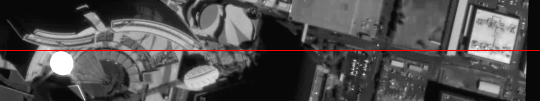
\includegraphics[width=\epiWidth\textwidth]{images/1519991772641_1st.png}\\
  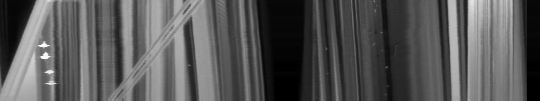
\includegraphics[width=\epiWidth\textwidth]{images/1519991772641_epi.png}\\
  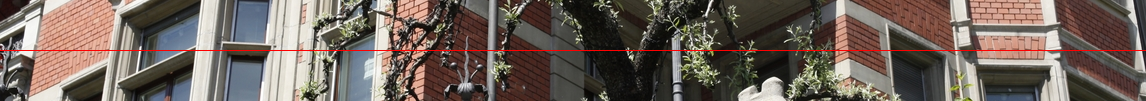
\includegraphics[width=\epiWidth\textwidth]{images/1521725699383_1st.png}\\[0.5cm]
  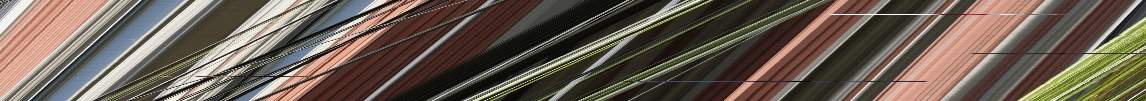
\includegraphics[width=\epiWidth\textwidth]{images/1521725699383_epi.png}
  \caption{Sample EPIs from SkysatLR18 (top) and MansionLR (bottom) datasets. We see that individual points leave a linear trace in the temporal dimension and that occlusions change over time.}
  \label{fig:exepi}
\end{figure}


\section{Description of the method}


\subsection{Disparity estimation from EPIs on confident points}


\paragraph{Principle} The main idea is, given a list of candidate disparities, to select the best slope for each point at which a confident measure can be done. Given a single line of an EPI, one first computes a confidence score. Then, for each confident point, one select the slope such that pixel radiances on the resulting line are the most densely distributed around a given mean radiance. This process is robust to occlusions.


\paragraph{Details} Let us consider some EPI $E$ corresponding to a fixed $v$, which dimensions are $s$ along the rows and $u$ along the columns. We work only on one line of this EPI at a time (beginning with the center line at $\widehat{s} = s_{\max} / 2$).



\begin{figure}[ht]
\centering
 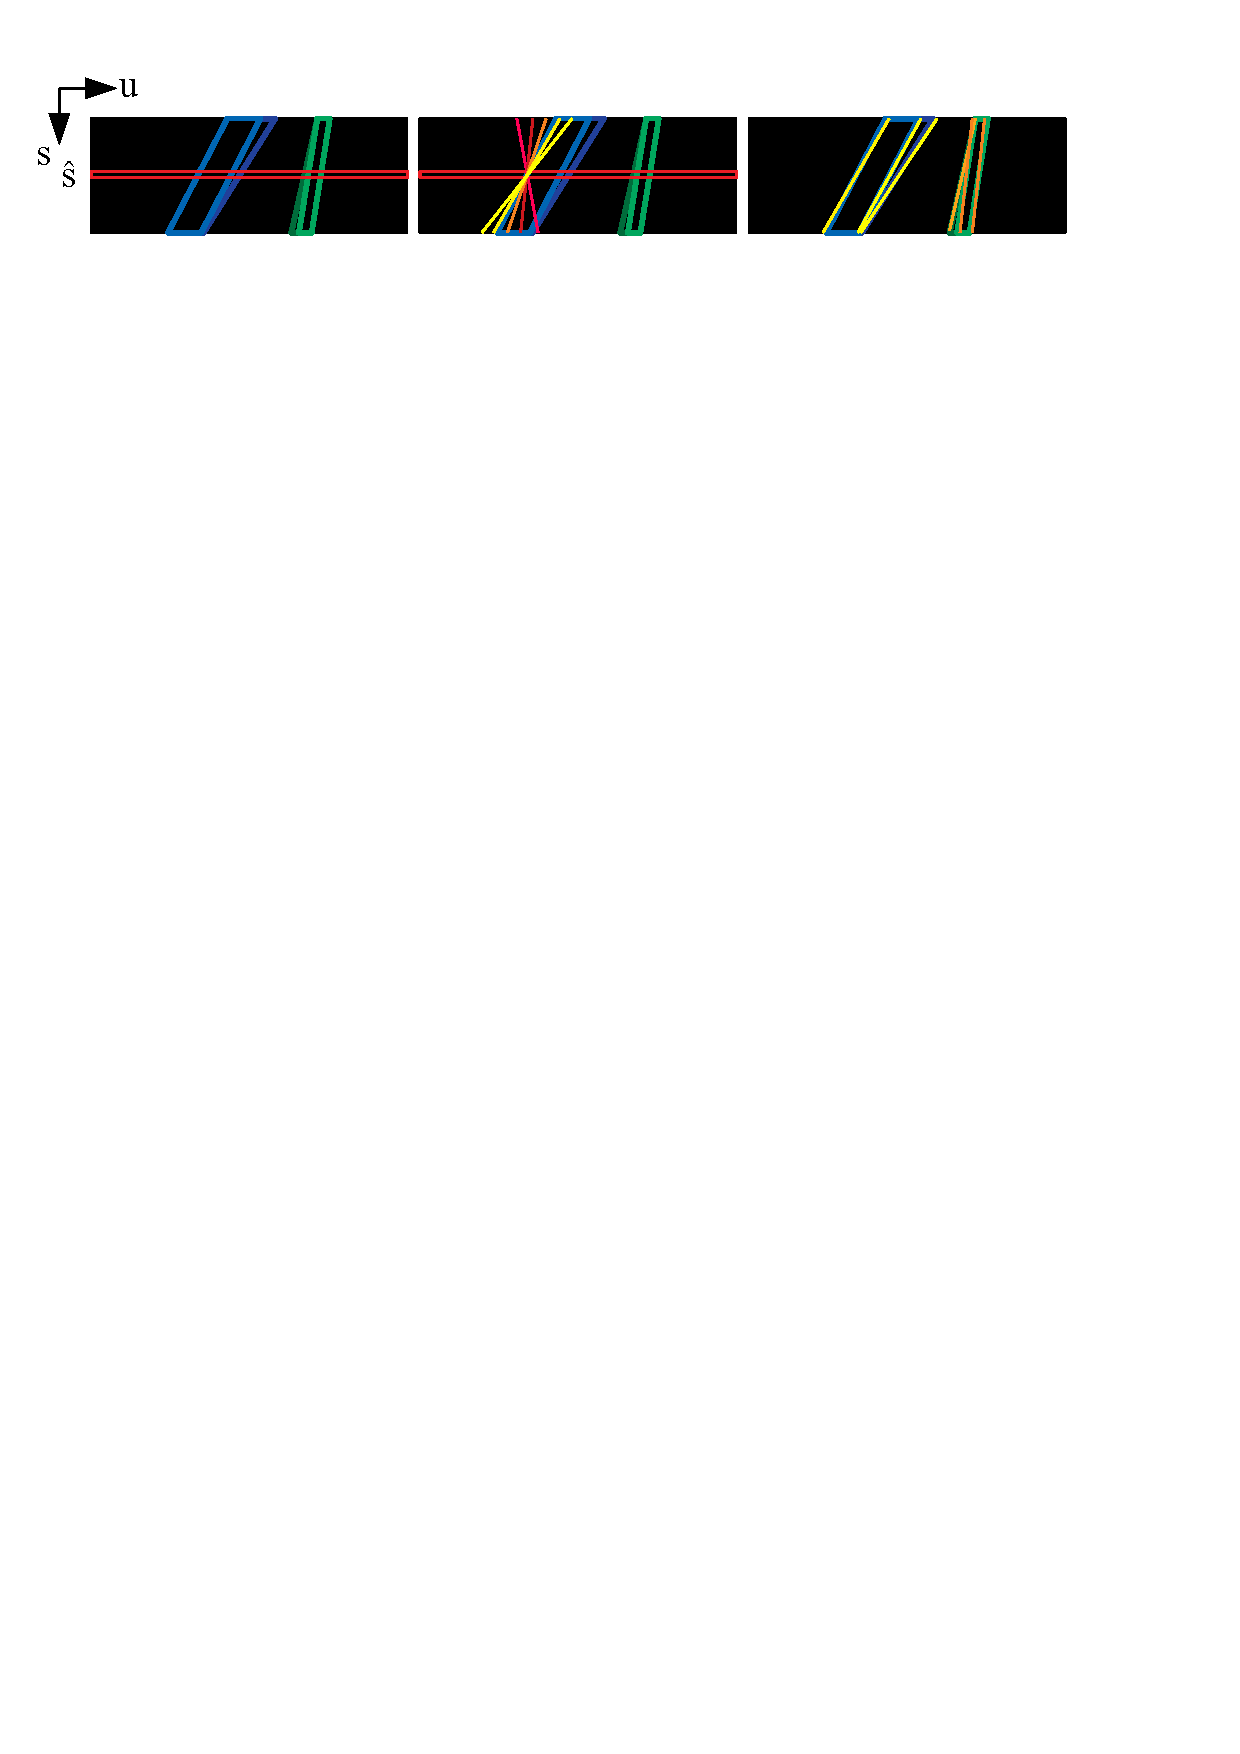
\includegraphics[width=1.0\textwidth, trim=0.5cm 26cm 2.5cm 1cm, clip]{drawings/depth_estimation.pdf}
 \caption{Disparity estimation process. Left: we select a row $\widehat{s}$. Middle: given a column $u$, we test several candidate $d$'s and select the one with the highest score $S(u, d)$. Right: we propagate the disparity along the temporal dimension for points belonging to  a confident edge, then repeat the process along each column $u$, and for every value $\widehat{s}$ if $d(\widehat{s}, u)$ was not computed yet.}
 \label{drawing:depth_estimation}
\end{figure}



To each point, we define an edge confidence measure $C_e$ such that
\begin{align}
 C_e (\widehat{s}, u) &= \sum_{u' \in \mathcal{N}_{C_e}(\widehat{s}, u)} \norm{E(\widehat{s}, u) - E(\widehat{s}, u')}^2. 
\end{align}
This measures diversity in the radiances of the image along a small linear window $\mathcal{N}_{C_e}(\widehat{s}, u)$ around the point $(\widehat{s}, u)$. It should be high on edges that show great color transitions and low on flat surfaces. The process is illustrated in Figure \ref{drawing:fine_to_coarse}.


The disparity estimation process is detailed in Figure \ref{drawing:depth_estimation}. Let $d_\text{list} = \left\{d_1, \cdots, d_D \right\}$ be a set of candidate disparities. We compute the set of radiances $\mathcal{R}$ of values of $E$ along the line centered on $u$ of slope $d$, for all confident couples $(u, d)$, i.e. at points $(\widehat{s}, u)$ such that $C_e(\widehat{s}, u) > \varepsilon_{C_e}$:
\begin{align} 
\mathcal{R}(u, d) &= \left\{ E(u + (\widehat{s} - s) d, s) \; | \; s = 0 \cdots S-1 \right\}.
\end{align}

We then compute a score $S(u, d)$ defined as:
\begin{align} 
S(u, d) = \frac{1}{\abs{\mathcal{R}(u, d)}} \sum_{\mathbf{r} \in \mathcal{R}(u, d)} K(\mathbf{r} - \overline{\mathbf{r}})
\end{align}
where $\mathbf{r}$ is a value $E(\cdot, \cdot)$, $\overline{\mathbf{r}}$ is some mean radiance value described hereafter, and $K$ is a ``kernel''. We choose the kernel presented in the article, i.e.
\begin{align}
K(\mathbf{r}) = \left\{ 
\begin{array}{l}
1 - \norm{\mathbf{r} / h}^2 \qquad \text{if $\norm{\mathbf{r} / h} < 1$} \\
0 \qquad \text{else}                            
\end{array} \right. .
\end{align}
We name this kernel the ``bandwidth kernel'' (where $h$ is a parameter). Its value is $0$ when $\norm{\mathbf{r}} \rightarrow +\infty$ and $1$ for $\norm{\mathbf{r}} \rightarrow 0$. Its role is to select $\mathbf{r}$ values that are reasonably near zero.

$\overline{\mathbf{r}}$ is a parameter that depends on $(u, d)$: following the article, we perform a truncated mean-shift algorithm (10 iterations), with $\overline{\mathbf{r}}_0 = E(u, \widehat{s})$ and
\begin{align} 
\overline{\mathbf{r}} \leftarrow \frac{\sum_{\mathbf{r} \in \mathcal{R}(u, d)} K(\mathbf{r} - \overline{\mathbf{r}}) \mathbf{r}}{\sum_{\mathbf{r} \in \mathcal{R}(u, d)} K(\mathbf{r} - \overline{\mathbf{r}})}
\end{align}
prior to the computation of $S(u, d)$, initializing with $\overline{\mathbf{r}} = E(\widehat{s}, u)$. The expected result is that $\overline{\mathbf{r}}$ will shift to the mean of the closest blob of radiances near $E(\widehat{s}, u)$, ignoring the values that are too far from this value (that are expected to be occlusions).


\paragraph{Technical difficulties} A line defined by $(u + (\widehat{s} - s) d, s)$ will very certainly have non-integer coordinates or go out of the image boundaries. We thus take the following decisions:
\begin{itemize}
 \item Values outside of the image are considered \emph{nan} and not taken into account in $\mathcal{R}(u, d)$.
 \item We have yet to decide on some proper interpolation method for computing non-integer values of $E$, for instance linear interpolation along the line $E(u, \cdot)$.
\end{itemize}


\subsection{Depth propagation along temporal axis}


For each $u$, we select the $d$ with the best score. We then propagate the disparities from $\widehat{s}$ to the other $(s', u')$ simply by drawing the depths along the lines $u' = u + (\widehat{s} - s)d$ if 
\begin{enumerate}
 \item $C_e(\widehat{s}, u) > \varepsilon_{C_e}$
 \item $C_e(s', u') > \varepsilon_{C_e}$
 \item $\norm{E(s', u') - E(\widehat{s}, u)} < \varepsilon_E$
\end{enumerate}
These points $(s', u')$ are marked as computed and not considered anymore. The algorithm then proceeds to new values $s$ that are close to $\widehat{s}$ (i.e. $s_{\max} / 2 + 1$, $s_{\max} / 2 - 1$, ...) and repeat the process.


After these steps, we obtain disparity values for each point such that $C_e$ was high enough, the other points having been masked.


\paragraph{Differences with the article} It should be noted that in \cite{art:kim13:lfields}, Kim et al. handle the situation in which a point with high edge confidence $C_e$ could have a bad disparity estimation $d$. This could for instance happen if the point is in the intersection of two lines of the same color with different slopes in the EPI. In order to do so, the authors define a disparity confidence score
\begin{align}
 C_d (\widehat{s}, u) &= C_e (\widehat{s}, u) \norm{\max_d S(u, d) - \mathrm{mean}_d S(u, d)}
\end{align}
and only retain and propagate $d$'s corresponding to points with a high $C_d$. We chose not to use this conservative criterion since it decreases significantly the number of valid estimations and tend to erase mildly sharp borders on buildings in our satellite images.


\subsection{Selective median filtering}


We repeat the process for all the lines $v$ -- since the process is independant for each $v$, this operation can be simultaneous.


When all lines $v$ have been computed, we apply a median filter on the resulting disparity map along dimensions $(v, u)$ such that in the end, for a point $(v, u)$ such that $C_e (v, u) > 0.02$, the selected value $d_{v, u}$ is the median value of the set:
\[ \left\{ d (v', u') \; | \; (v', u') \in \mathcal{N}_\text{sel. median}(v, u), \; C_e(v', u') > \varepsilon_{C_e}, \; \norm{E_{v}(\widehat{s}, u) - E_{v'}(\widehat{s}, u')} < \varepsilon_{E} \right\}.\]

$\mathcal{N}_\text{sel. median}(v, u)$ is a neighbourhood of $(v, u)$. The expected result is to filter speckles among points of the same color that are also close one to the other. After this step, all the disparities have been computed and filtered in points $(s, v, u)$ such that $C_e(s, v, u)$ was high enough.


\subsection{Fine-to-coarse approach}


The approach presented in \cite{art:kim13:lfields} is based on a ``fine to coarse'' approach. It consists in making confident disparity estimations in the images for different spatial scales $(v, u)$ and recombining these disparities in order to reconstruct a complete disparity map at the finest scale.


In order to proceed to a multi-scale analysis, the idea is to use the regularizing effect of downsampling. We thus create a pyramid of downsampled images, with coarser and coarser disparity estimations. The confident estimations at the finest scale are likely to be made on small objects or contours, whereas the estimations at the coarser scales will be related to plain surfaces for instance. The algorithm will then merge the estimations computed at the different scales by sequentially filling the blank estimations back from coarse to fine by upsampling disparity maps at a given scale to the preceding finer scale. This process is presented in Figure \ref{drawing:fine_to_coarse}.



\begin{figure}[ht]
\centering
 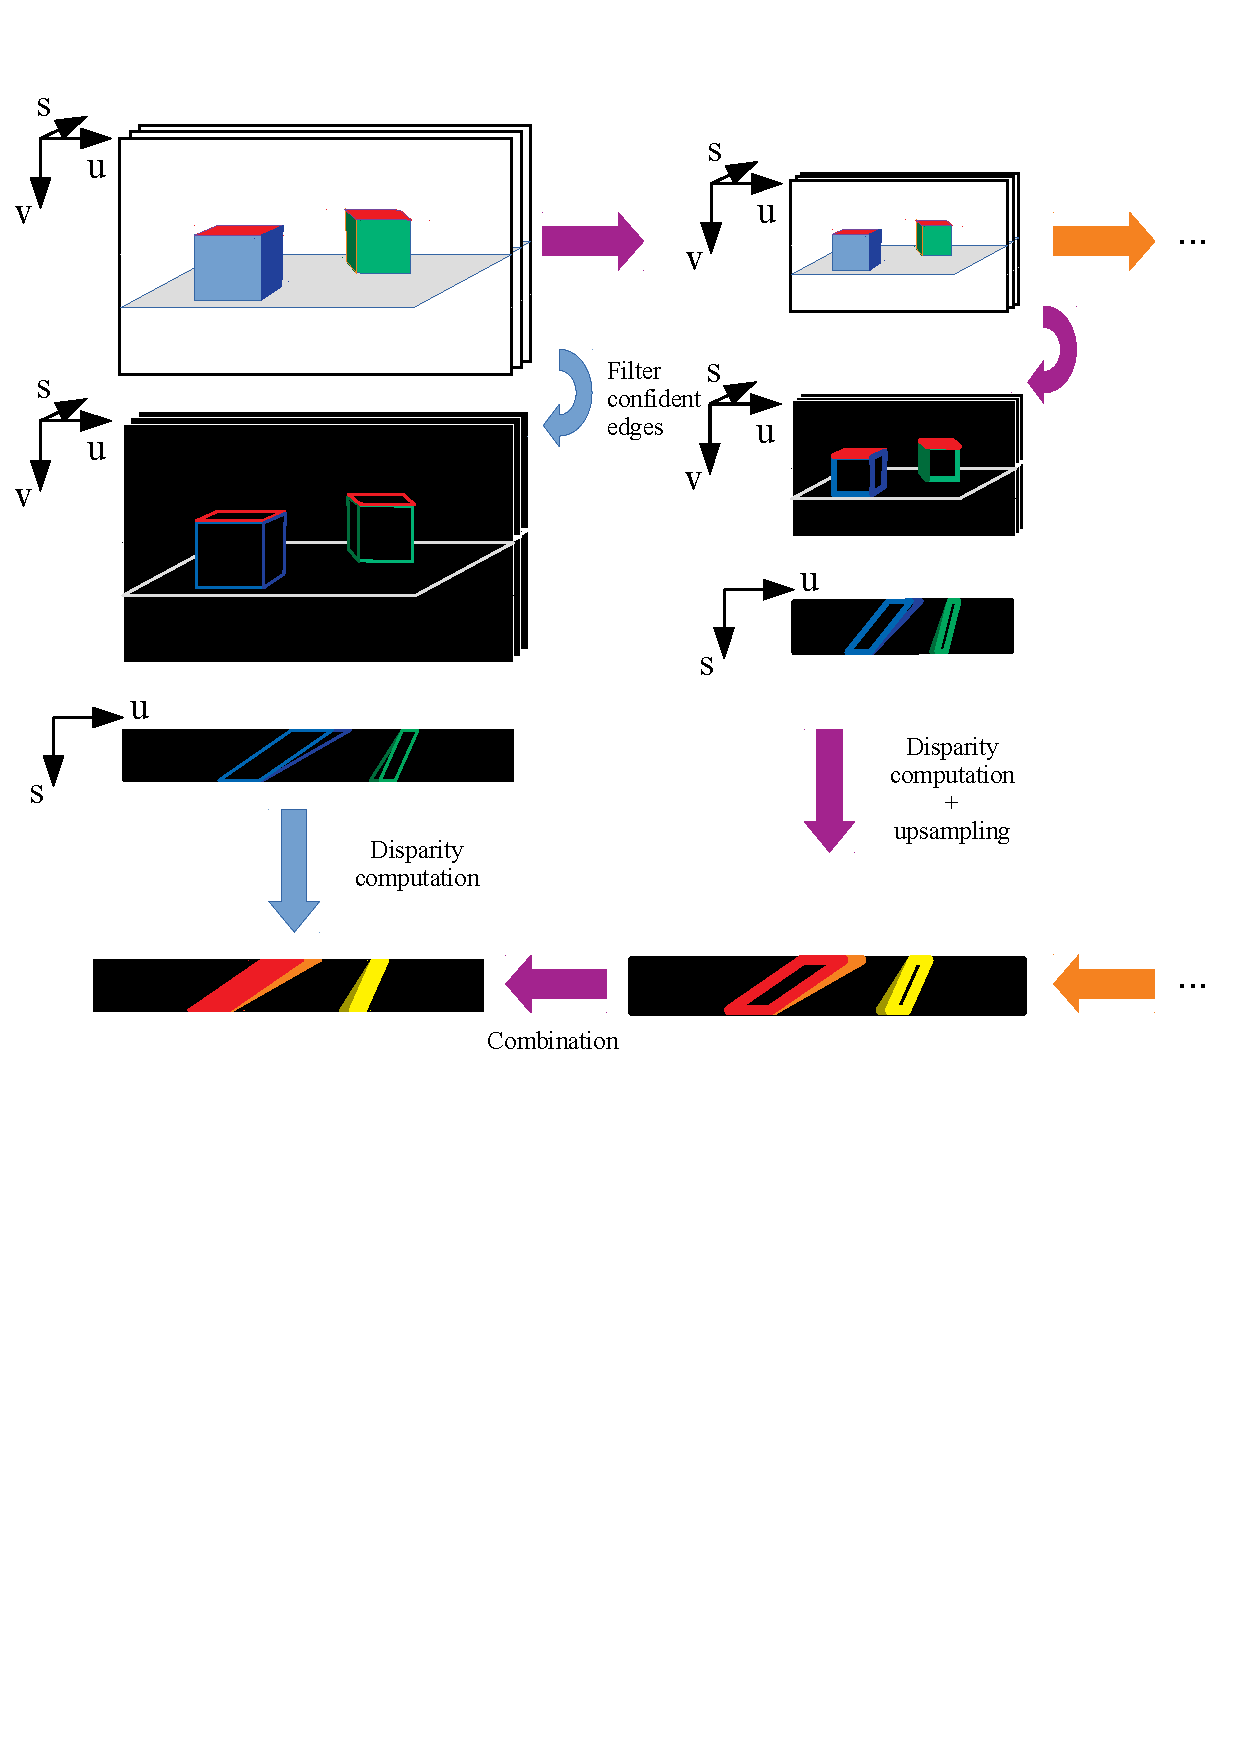
\includegraphics[width=1.0\textwidth, trim=0cm 11cm 0cm 0.5cm, clip]{drawings/fine_to_coarse.pdf}
 \caption{Fine to coarse approach.}
 \label{drawing:fine_to_coarse}
\end{figure}



\paragraph{Downsampling} We progressively fill the zones left blank by our confidence criterion (we choose here $C_e > \varepsilon_{C_e}$ ; one could apply $C_d > \varepsilon_{C_d}$ like in the article but this is significantly more conservative). This approach is similar to building a pyramid of images, and writes as follow:
\begin{enumerate}
 \item Let us consider a pile of images at the scale $p$ (the ``stair $p$'' of the pyramid). One first applies a Gaussian filter in the spatial dimensions $(v, u)$ with window $\mathcal{N}_\text{downsampling}$.
 \item We then downsample the images by taking one line over 2 in the spatial dimensions $(v, u)$ ; the resolution along the temporal dimension $s$ is left unchanged. This is the stair $p+1$ of the pyramid of images.
 \item Then, we use the confident disparities computed at the scale $p$ in order to derive disparity bounds for the scale $p+1$. This step is not described precisely in the article ; we chose, given a point $(s, v', u')$ in $p+1$, to select the 2 pairs of points $(s, v, [u_1^1, u_2^1])$ $(s, v+1, [u_1^2, u_2^2])$ where $v = 2 v'$ and $u_1^1$, $u_1^2$ are the first confident points at the left and right of $u=2u'$. The bounds for $(s, v', u')$ will be the $\min$ and the $\max$ disparities among these points.
 \item We then perform a disparity computation along all axis as described in the preceding section.
\end{enumerate}
The pyramid process is represented in Figure \ref{fig:pyramid}. The confidence score will be less and less restrictive due to the regularization effect of downsampling.


\begin{figure}[th]
  \centering
  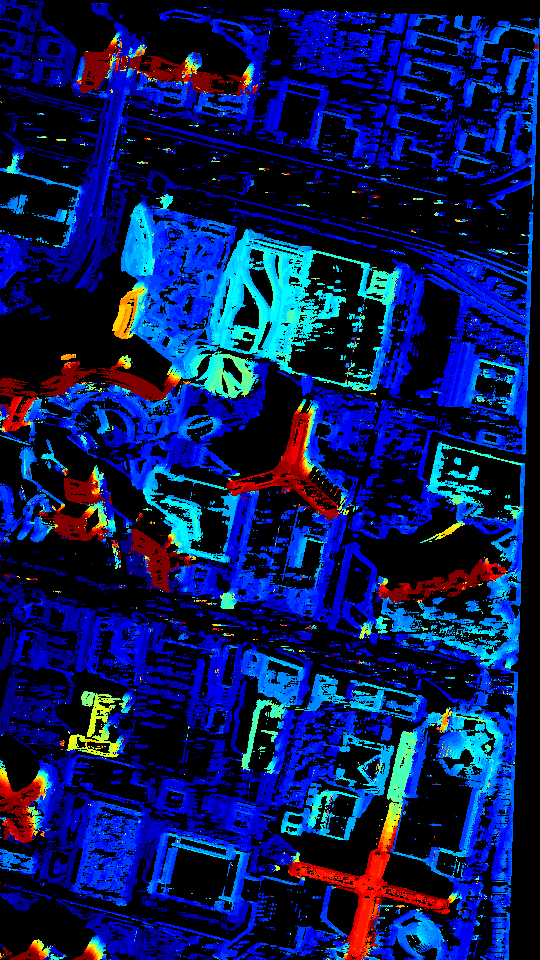
\includegraphics[width=0.4\textwidth]{images/pyr/1521741442733_pyr_depth_000.png}
  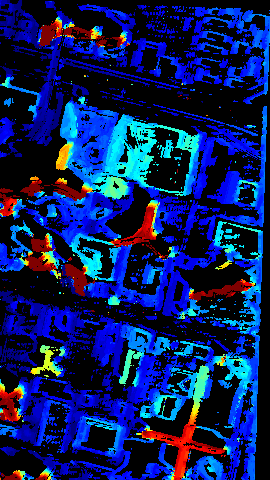
\includegraphics[width=0.2\textwidth]{images/pyr/1521741442733_pyr_depth_001.png}
  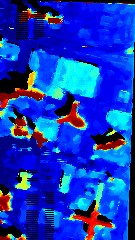
\includegraphics[width=0.1\textwidth]{images/pyr/1521741442733_pyr_depth_002.png}
  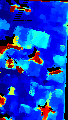
\includegraphics[width=0.05\textwidth]{images/pyr/1521741442733_pyr_depth_003.png}
  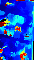
\includegraphics[width=0.025\textwidth]{images/pyr/1521741442733_pyr_depth_004.png}
  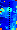
\includegraphics[width=0.0125\textwidth]{images/pyr/1521741442733_pyr_depth_005.png} \\
  
\includegraphics[width=0.4\textwidth]{images/pyr/1521741442733_pyr_epi_000.png}
  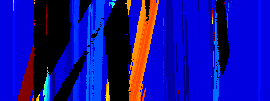
\includegraphics[width=0.2\textwidth]{images/pyr/1521741442733_pyr_epi_001.png}
  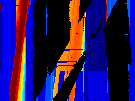
\includegraphics[width=0.1\textwidth]{images/pyr/1521741442733_pyr_epi_002.png}
  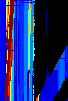
\includegraphics[width=0.05\textwidth]{images/pyr/1521741442733_pyr_epi_003.png}
  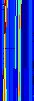
\includegraphics[width=0.025\textwidth]{images/pyr/1521741442733_pyr_epi_004.png}
  
\includegraphics[width=0.0125\textwidth]{images/pyr/1521741442733_pyr_epi_005.png}
  \\[0.5cm]
  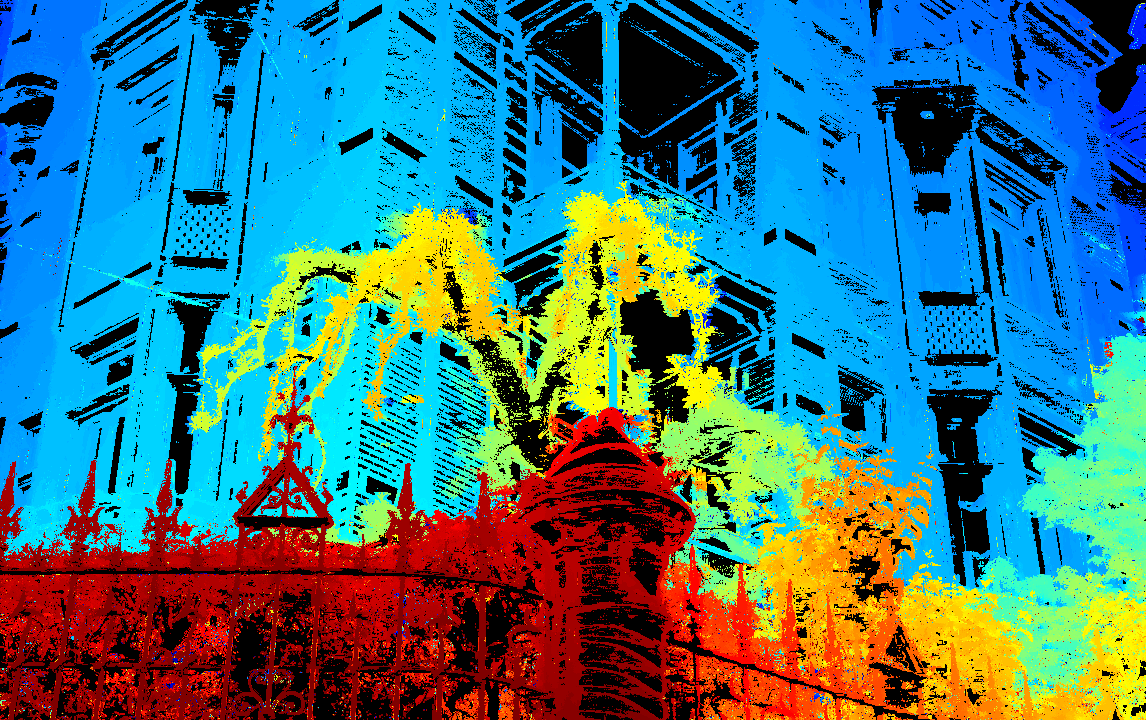
\includegraphics[width=0.4\textwidth]{images/pyr/1521751973001_pyr_depth_000.png}
  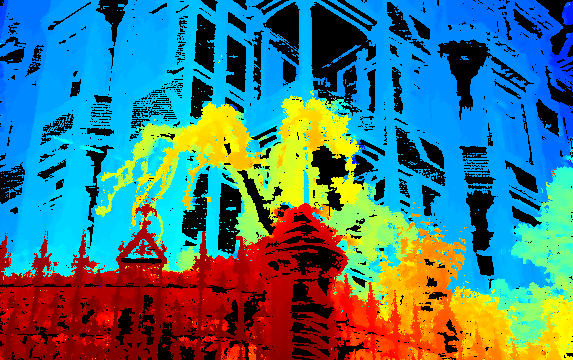
\includegraphics[width=0.2\textwidth]{images/pyr/1521751973001_pyr_depth_001.png}
  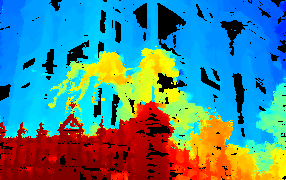
\includegraphics[width=0.1\textwidth]{images/pyr/1521751973001_pyr_depth_002.png}
  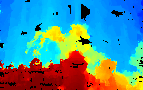
\includegraphics[width=0.05\textwidth]{images/pyr/1521751973001_pyr_depth_003.png}
  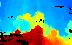
\includegraphics[width=0.025\textwidth]{images/pyr/1521751973001_pyr_depth_004.png}
  
\includegraphics[width=0.0125\textwidth]{images/pyr/1521751973001_pyr_depth_005.png}
  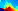
\includegraphics[width=0.00625\textwidth]{images/pyr/1521751973001_pyr_depth_006.png}\\
  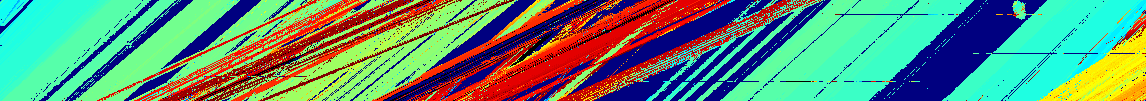
\includegraphics[width=0.4\textwidth]{images/pyr/1521751973001_pyr_epi_000.png}
  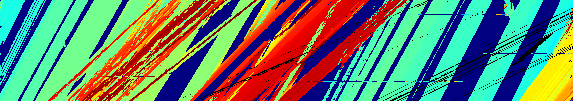
\includegraphics[width=0.2\textwidth]{images/pyr/1521751973001_pyr_epi_001.png}
  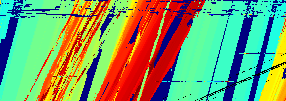
\includegraphics[width=0.1\textwidth]{images/pyr/1521751973001_pyr_epi_002.png}
  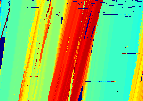
\includegraphics[width=0.05\textwidth]{images/pyr/1521751973001_pyr_epi_003.png}
  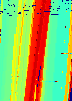
\includegraphics[width=0.025\textwidth]{images/pyr/1521751973001_pyr_epi_004.png}
  
\includegraphics[width=0.0125\textwidth]{images/pyr/1521751973001_pyr_epi_005.png}
  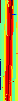
\includegraphics[width=0.00625\textwidth]{images/pyr/1521751973001_pyr_epi_006.png}
  \caption{Pyramid of downsampled disparity maps and sample EPIs (after disparity computation) for the Skysat sequence with step 18 (SkysatLR18, top) and mansion sequence (MansionLR, bottom).}
  \label{fig:pyramid}
\end{figure}


\paragraph{Going back up to the finest scale} In order to retrieve the disparity map to the finest scale $p=0$, one then proceeds the other way round:
\begin{enumerate}
 \item Starting at $p=p_{\max}$, one upscales the disparity estimates (with bilinear interpolation) and the validity mask $M_e = \{C_e > \varepsilon_{C_e}\}$ (with nearest neighbour interpolation).
 \item Consider the disparity map at scale $p-1$. Fill the blank zones of this disparity map using the upscaled disparity map from $p$ at confident points from $M_e$.
\end{enumerate}


In the end, following the paper, we also make the following refinements:
\begin{itemize}
 \item We apply a median filter on the final disparity map estimates with window $\mathcal{N}_\text{fin. median}$.
 \item When establishing the map of valid points $M_e = \{C_e > \varepsilon_{C_e}\}$, one can perform a mathematical opening in order to remove falsely confident points. We find out that this degrades the performance of the algorithm on non-sharp images such as the Skysat sequence, so we chose to deactivate this feature.
\end{itemize}


\clearpage
\section{Results}


\subsection{Datasets and parameters}


The parameters we used for the following results are presented in Table \ref{table:parameters}. We chose to test our algorithm on the original data of \cite{art:kim13:lfields} along with satellite images taken from a public Skysat video. The datasets are described in Table \ref{table:datasets}.


\paragraph{Parameters and number of channels} It should be noted that MansionLR is a tri-channel dataset and Skysat is a mono-channel dataset. Our kernels, confidence measure and color thresholds use the Euclidean norm of the values of images -- in order to use the same parameters for all the experiments and maintain coherence between the experiments, we decide to define the parameters for tri-channel images and redefine the Euclidean norm for the mono-channel images as follows:
\begin{align}
 \forall x \in \R, \qquad \norm{x} &= \sqrt{3} \times \abs{x}.
\end{align}
We could also redefine the norm for quad-channel images for instance with a factor $\sqrt{3/4}$.


\paragraph{Preprocessing normalization} Images can be given in the tricolor format $(0\cdots 255)^3$ or in \verb#float# format. We decide to convert all the EPIs in \verb#float# as a preprocessing and scale the values by a factor $255$ if the image was in \verb#uchar#, or so that the maximum is $1.0$ if the image was given in \verb#float#. 


\paragraph{Shading} Satellite images show numerous dark zones due to shading. These zones are homogeneous and non-textured, so that no clear disparity estimation can be done -- we decide to mask these zones both during the disparity estimation process and in the final disparity maps. We thus ignore zones such that $\norm{E} < 0.05 \sqrt{3}$.


\paragraph{Colors and plots} We use the \verb#colormap#s of OpenCV\footnote{\url{https://docs.opencv.org/3.4.1/d3/d50/group__imgproc__colormap.html}} in our plots. In the following, we mainly use the \verb#JET# colormap.%, and sometimes the \verb#HOT# colormap.



\begin{table}[ht]
 \centering
 \begin{tabular}{|c|l|l|}
  \hline
  \textbf{Parameter} & \textbf{Description} & \textbf{Value}\\
  \hline \hline 
  $\mathcal{N}_{C_e}$ & $C_e$ computation window. &  Horizontal window of size $9$.\\
  \hline 
  $h$ & Bandwith kernel parameter. & 0.2 \\
  \hline 
  $\varepsilon_{C_e}$ & Confidence edge threshold. & 0.02 \\
  \hline 
  $\varepsilon_E$ & Color difference propagation threshold. & 0.1 \\
  \hline 
  $\mathcal{N}_\text{sel. median}$ & Selective median filter window. & Square centered neighbourhood of size $11$. \\
  \hline 
  $\mathcal{N}_\text{downsampling}$ & Downsampling gaussian filter window. & Square centered neighbourhood of size $7$.\\
  \hline 
  $\mathcal{N}_\text{fin. median}$ & Final median filter window. & Square centered neighbourhood of size $3$.\\
  \hline
 \end{tabular}
 \caption{Values of the parameters used}
 \label{table:parameters}
\end{table}

\begin{savenotes}
\begin{table}[ht]
 \centering
 \begin{tabular}{|c|p{10cm}|}
  \hline
  \textbf{Dataset} & \textbf{Description} \\
  \hline \hline 
  MansionLR &Mansion preprocessed dataset\footnote{\url{http://people.csail.mit.edu/changil/publications/scene-reconstruction-from-high-spatio-angular-resolution-light-fields-siggraph-2013-datasets.html}}, that we resize to a resolution of $1146\times 720$\\
  \hline 
  SkysatLR18 & Satellite images taken from a public Skysat video\footnote{\url{https://www.youtube.com/watch?v=lKNAY5ELUZY}} that we rectify. We proceeded first with a version downsampled to $540\times 960$ using one frame every $18$ frames.\\
  \hline 
  SkysatLR01 & Same as SkysatLR18 but taking every frame.\\
  \hline 
  SkysatHR18 & Same as SkysatLR18 but using the original $1080\times 1920$ resolution.\\
  \hline
 \end{tabular}
 \caption{Datasets and runtimes. Each dataset sequence is of length $100$ (i.e. $s=0\cdots 99$). }
 \label{table:datasets}
\end{table}
\end{savenotes}


\begin{table}[ht]
\centering
  \begin{tabular}{|c|c|c|}
   \hline
  \textbf{Dataset} & \textbf{Candidate $d$'s} & \textbf{Runtime (s)}\\
  \hline \hline 
  \multirow{2}{*}{MansionLR} & $0:4$ $[120]$ & $7409$\\
  & $0:4$ $[240]$ & ???\\
  \hline 
  \multirow{2}{*}{SkysatLR18} & $-1:4$ $[120]$ & $448$\\
  & $-1:4$ $[240]$ & $804$\\
  \hline 
  \multirow{2}{*}{SkysatLR01} & $-0.5:0.5$ $[120]$ & $143$\\
  & $-0.5:0.5$ $[240]$ & $254$\\
  \hline 
  \multirow{2}{*}{SkysatHR18} & $-2:8$ $[120]$ & ???\\
  & $-2:8$ $[240]$ & $2888$\\
  \hline
  \end{tabular}

 \caption{Tests and runtimes. Candidate $d$'s are indicated by $\mathrm{range}[\text{number of values}]$. Computations were run on a desktop Intel Core i3-6100 (2 cores, 4 threads @3.70 Ghz) with $16$ Gb of RAM.}
 \label{table:tests}
\end{table}




\subsection{Validation on the original dataset and qualitative results}


\paragraph{Validation} We perform the depth estimation on one of the original datasets of Kim et al. (MansionLR) and compare our disparity map to theirs. The results are presented in Figure \ref{fig:comparison_kim}. As expected, our results are less precise, noticeably behind the tree (that is partially merged with the wall behind it). This can be explained by the fact that we used images of 8 MP (compared to 19 MP) and did not implement the conservative criterion $C_d$ on disparity confidence (that result in more artefacts in the final estimation). The results are quite similar on other zones: the main structures seem correctly detected and estimated, especially the foliage at the right, the tree branch silhouettes in the center, the barrier at the front and the flat surfaces on the mansion wall. This validates the pertinence and efficiency of the fine-to-coarse approach.


\begin{figure}[ht]
 \centering
 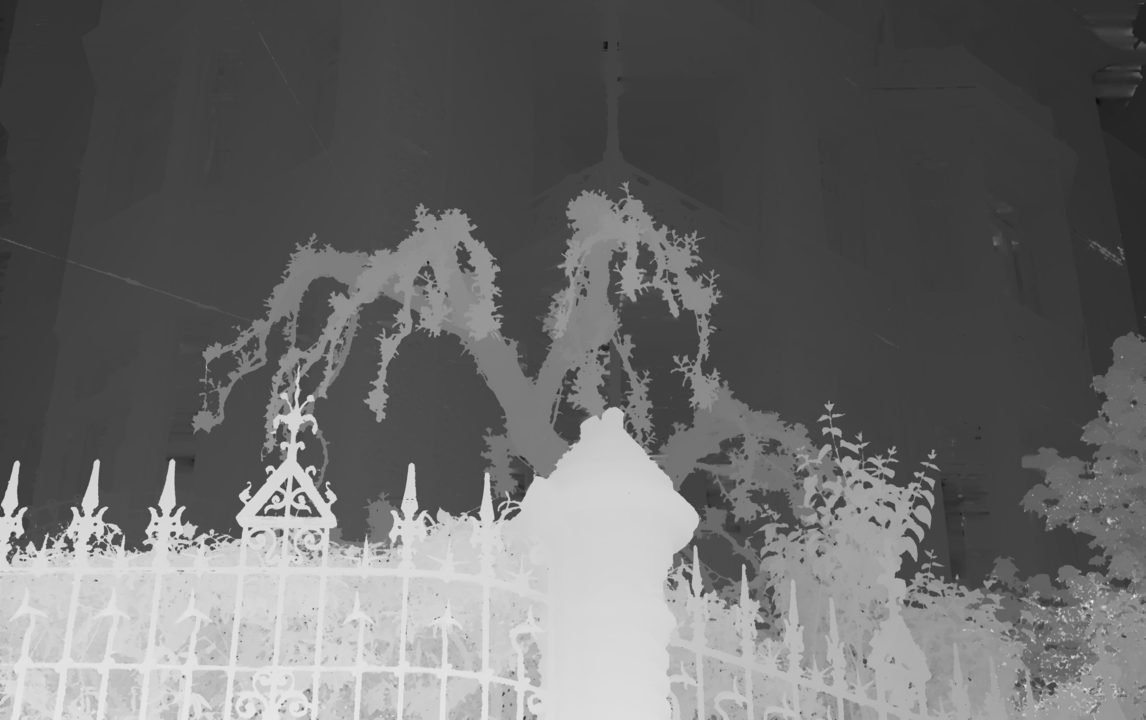
\includegraphics[width=0.9\textwidth]{images/mansion_kim_resized.png}
 \caption{Comparison of the results of Kim et al. in \cite{art:kim13:lfields} (top, computed using high definition images) and ours (bottom, computed with MansionLS, with $d=0:4$ $[240]$).}
 \label{fig:comparison_kim}
\end{figure}




\paragraph{Limitations} The fact that we define new disparity bounds at each step ensures the coherence of the depth estimations when the depth at the boundaries of an object have been computed. It should be noted that the best estimates are made for frames near $\widehat{s} = \dim s / 2$ as the propagation process might end up perturbating the estimates. This is due to changes in the image such as:
\begin{itemize}
 \item New objects appearing, objects disappearing.
 \item Objects changing shape (for instance, the walls of a building are likely to change shape due to perspective effects).
 \item Global changes in illumination conditions. This is notable in the Skysat dataset.
 \item Shading. This appears to be a great source of errors in the Skysat dataset, as the shadows will be interpreted as rough confident edges, but are not textured, so their depth estimates will be flawed. We decided to remove the shadow areas by setting the pixels with $\norm{E(s, v, u) < 0.05}$ to $C_e = 0$.
 \item Tricky surfaces such as reflective surfaces (the glass surfaces on buildings) will be misinterpreted since they reflect the ground... and thus will have a disparity dependant on the viewpoint of the camera, with a negative sign.
\end{itemize}


\paragraph{On a sequence with small slopes}


We investigate the performance of the algorithm with very small slopes with a sequence of Skysat with slower variations. A sample EPI is presented in Figure \ref{fig:epi:skysat1}. This example is harder since the variations are mostly under the scale of a pixel. We ran the algorithm with a choice of $d_{\min} = -0.5$ to $d_{\max} = 0.5$ and $120$ steps. Some results are presented in Figure \ref{fig:skysatlr01:candidated}. These results are quite satisfactory given the small slopes to be measured, but show globally some underestimated slopes on the top of the buildings. We assume these are due to the fact that the disparities are harder to be estimated when undersampling - these may be improved by using better interpolation formulae.


\begin{figure}[ht]
  \centering
  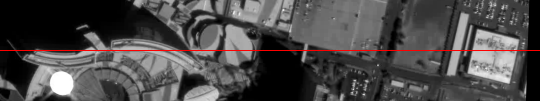
\includegraphics[width=\epiWidth\textwidth]{images/1521592293547_1st.png}\\
  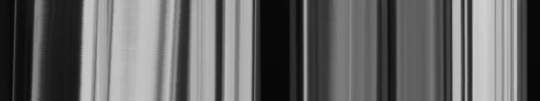
\includegraphics[width=\epiWidth\textwidth]{images/1521592293547_epi.png}
  \caption{Sample EPI from the Skysat sequence with slow variations.}
  \label{fig:epi:skysat1}
\end{figure}


\subsection{Influence of the candidate disparities}


We compare the results for the same frames of the same datasets with a number of $120$ and $240$ candidate $d$'s between the same bounds to evaluate the influence of the candidate $d$ set on the results. The results are presented in Figures \ref{fig:skysatlr18:candidated}, \ref{fig:skysatlr01:candidated} and xxx.


\begin{figure}[ht]
 \centering
 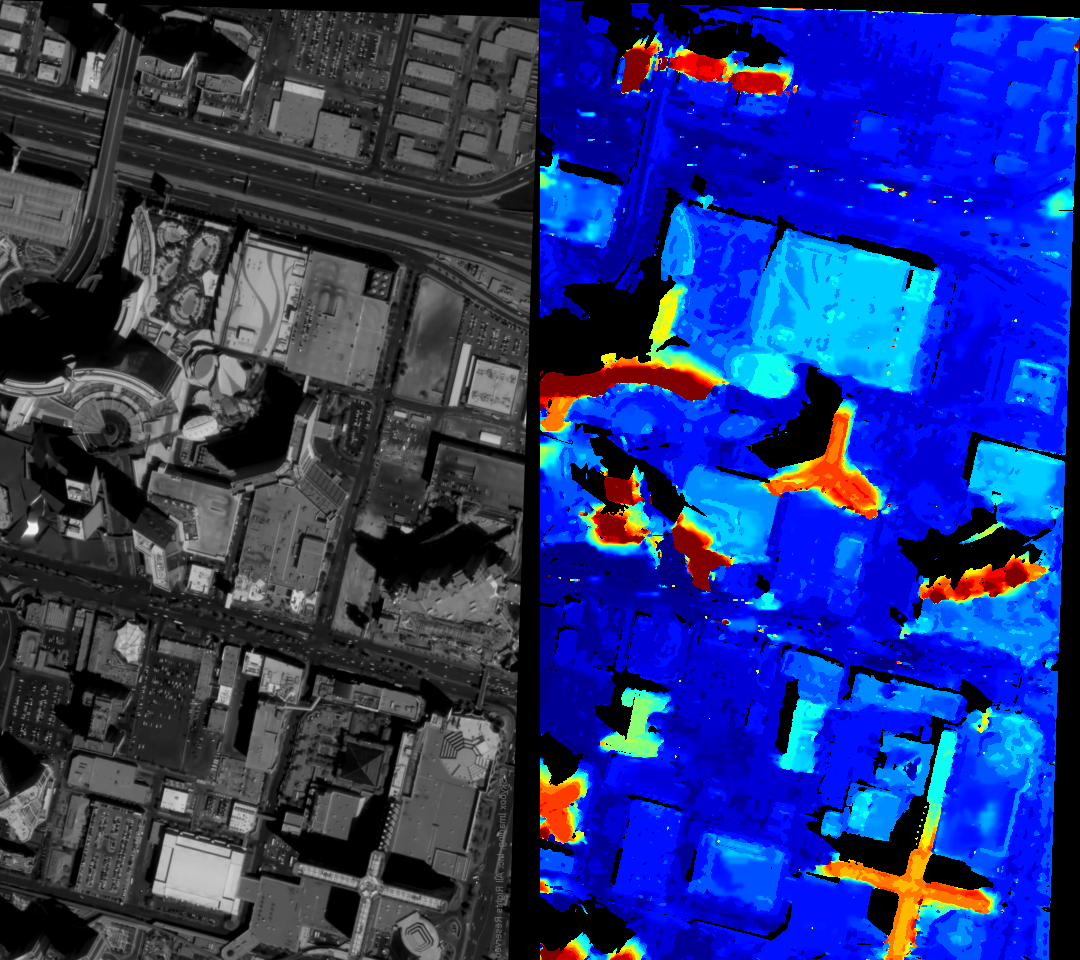
\includegraphics[height=8cm]{images/SkysatLR18_120/1521739947374_dmap_050.png}\hspace{-0.28em}
 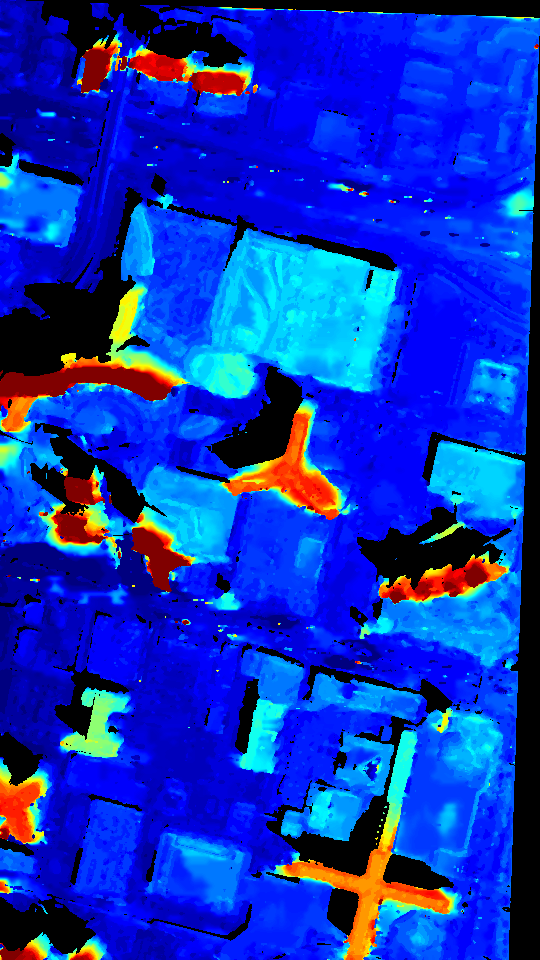
\includegraphics[height=8cm]{images/SkysatLR18_240/1521741442733_dmap_050.png}\\
 \vspace{-0.11em}
 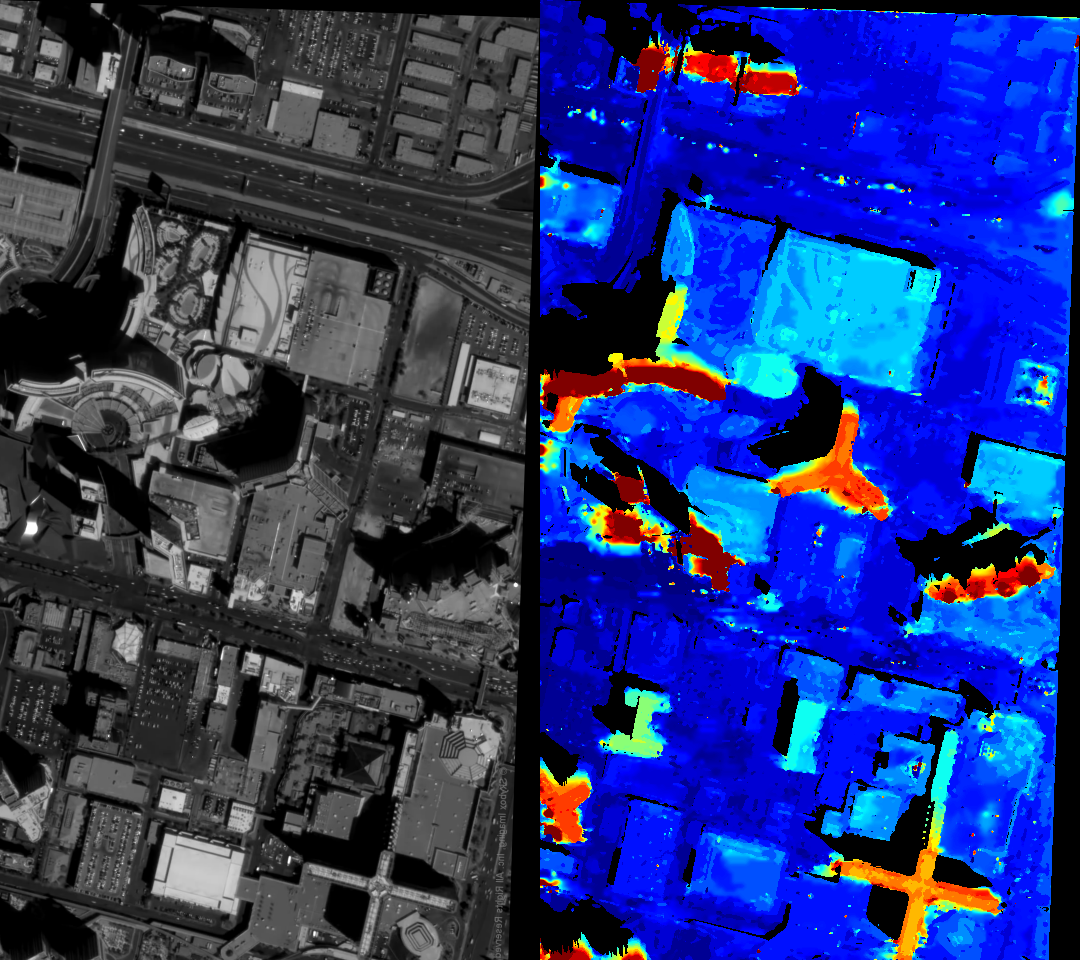
\includegraphics[height=8cm]{images/SkysatLR18_120/1521739947374_dmap_025.png}\hspace{-0.28em}
 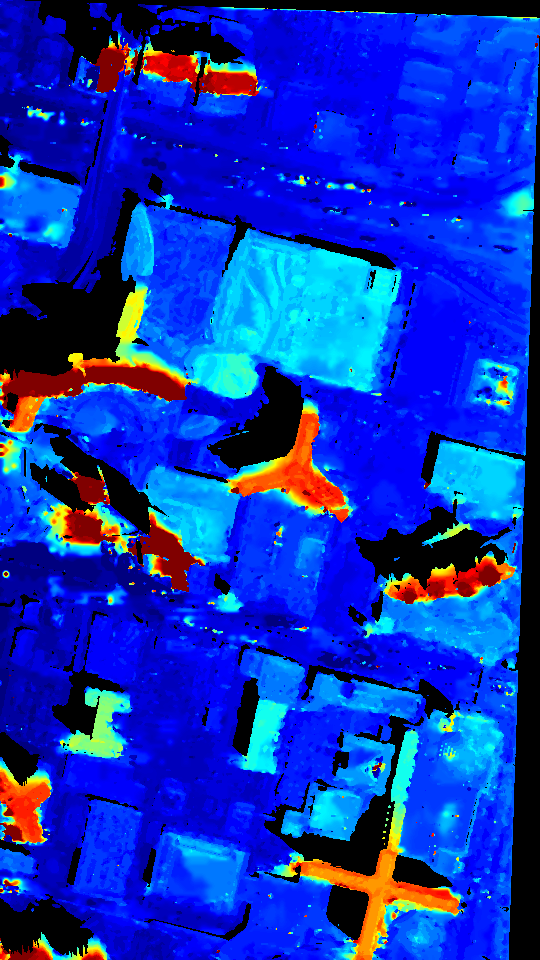
\includegraphics[height=8cm]{images/SkysatLR18_240/1521741442733_dmap_025.png}
 \caption{Influence of the candidate disparities. SkysatLR18, original frame (left) $-1:4$ $[120]$ (middle) and $-1:4$ $[240]$ (right). Frame $50$ (top) and $25$ (bottom).}
 \label{fig:skysatlr18:candidated}
\end{figure}


\begin{figure}[ht]
 \centering
 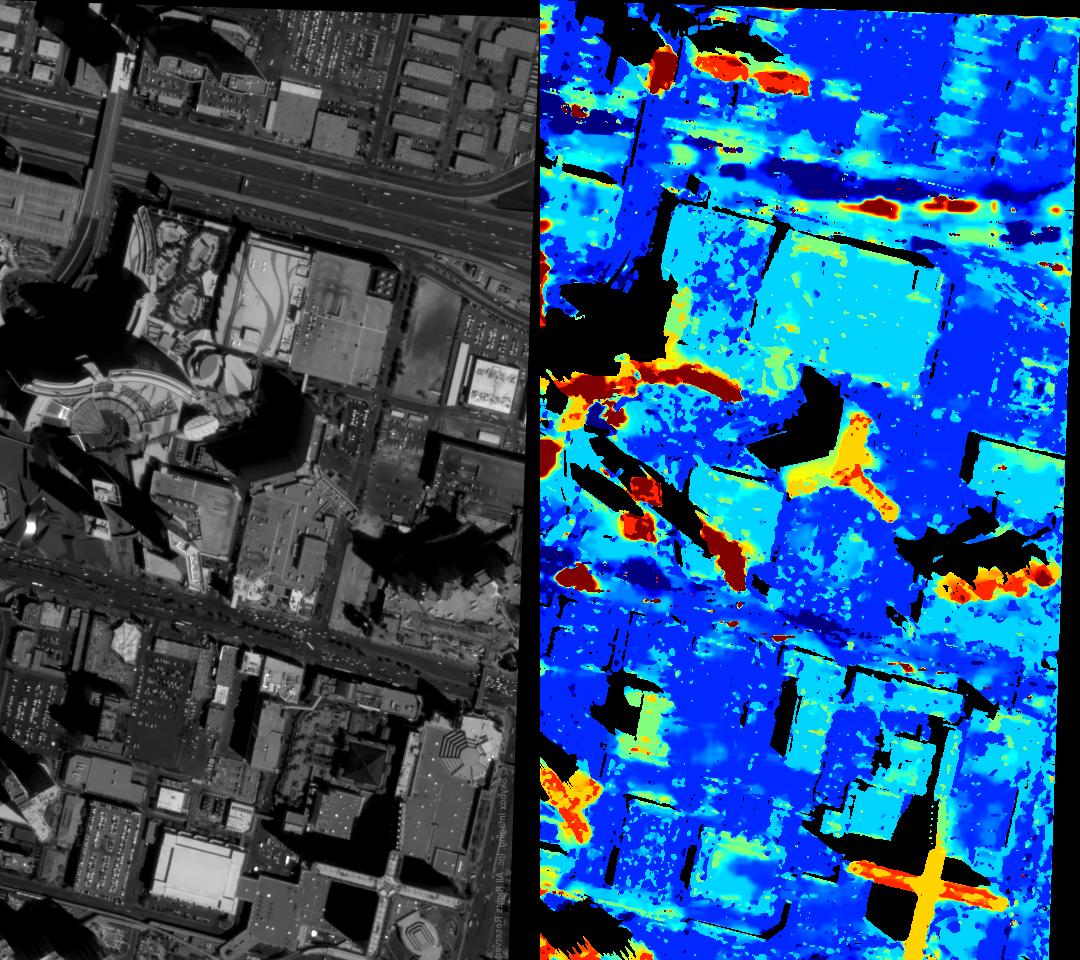
\includegraphics[height=8cm]{images/SkysatLR01_120/1521737975374_dmap_050.png}\hspace{-0.28em}
 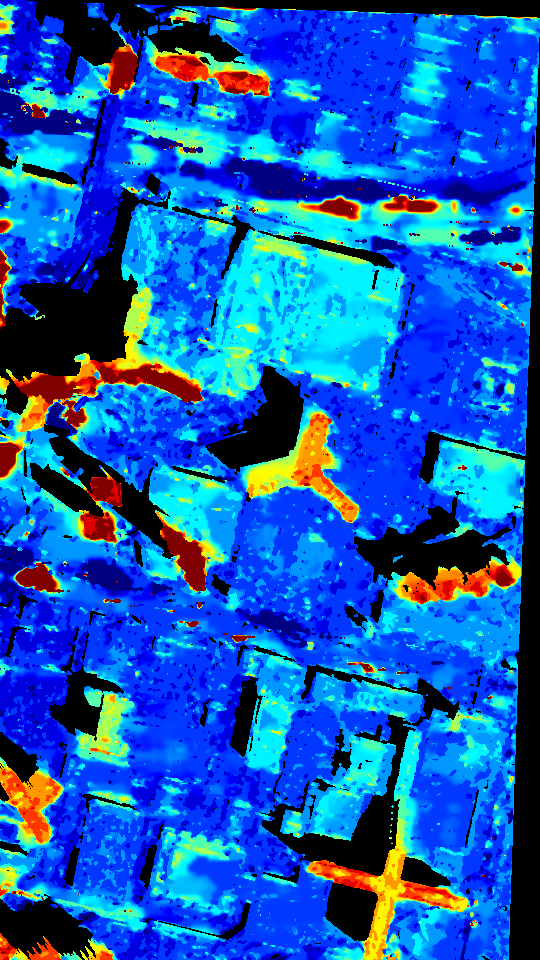
\includegraphics[height=8cm]{images/SkysatLR01_240/1521738847855_dmap_050.png}\\
 \vspace{-0.11em}
 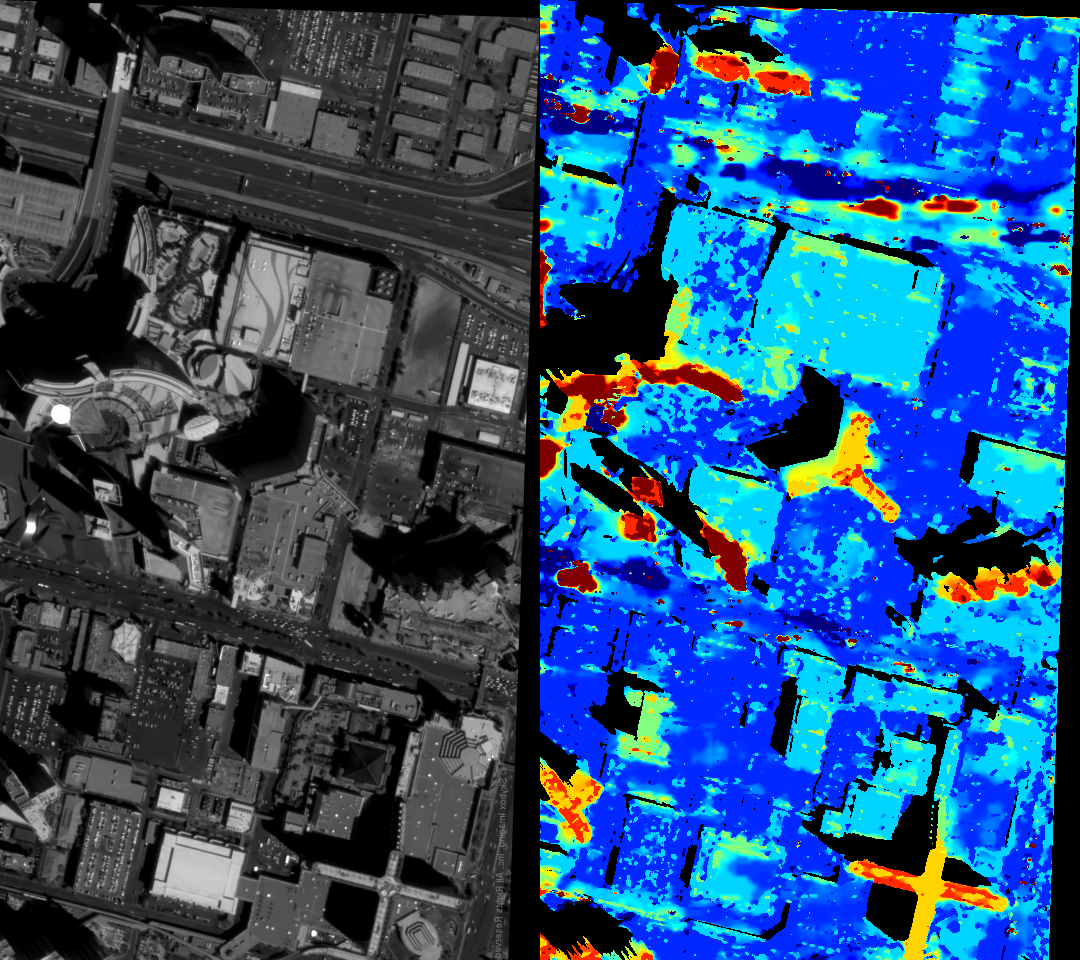
\includegraphics[height=8cm]{images/SkysatLR01_120/1521737975374_dmap_025.png}\hspace{-0.28em}
 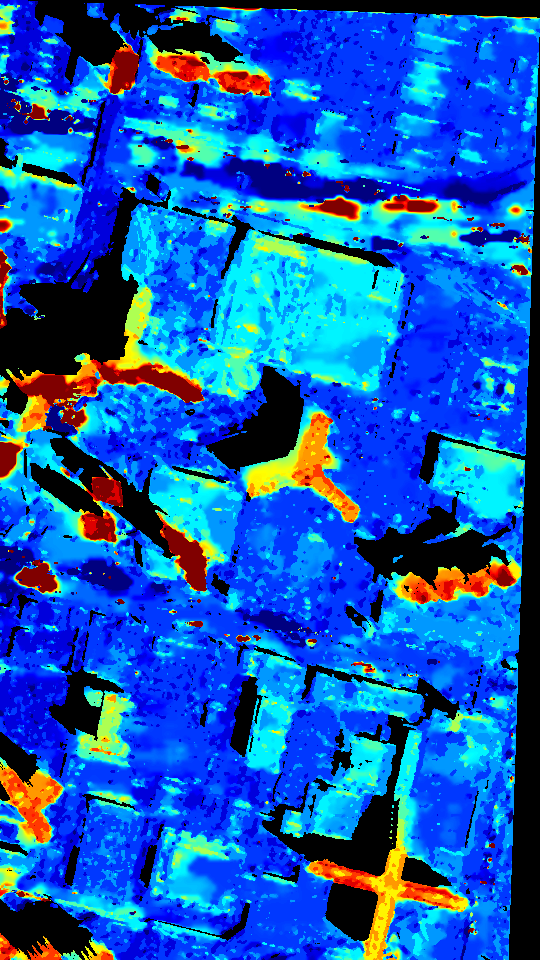
\includegraphics[height=8cm]{images/SkysatLR01_240/1521738847855_dmap_025.png}
 \caption{Influence of the candidate disparities. SkysatLR01, original frame (left) $-1:4$ $[120]$ (middle) and $-1:4$ $[240]$ (right). Frame $50$ (top) and $25$ (bottom).}
 \label{fig:skysatlr01:candidated}
\end{figure}


\subsection{Influence of the resolution}


We compute the disparity estimations on the same frame Figure \ref{fig:influenceres}


\begin{figure}[ht]
 \centering
 %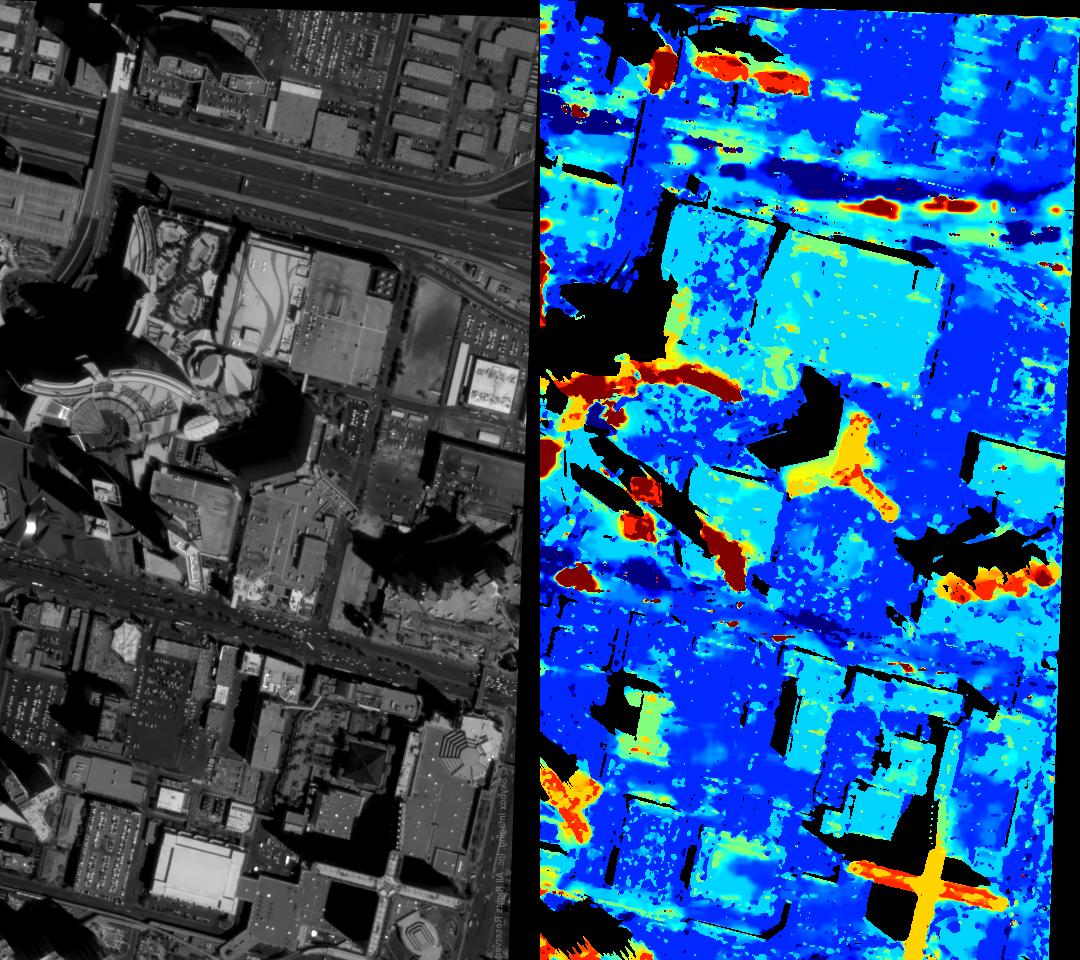
\includegraphics[height=8cm]{images/SkysatLR01_120/1521737975374_dmap_050.png}\hspace{-0.28em}
 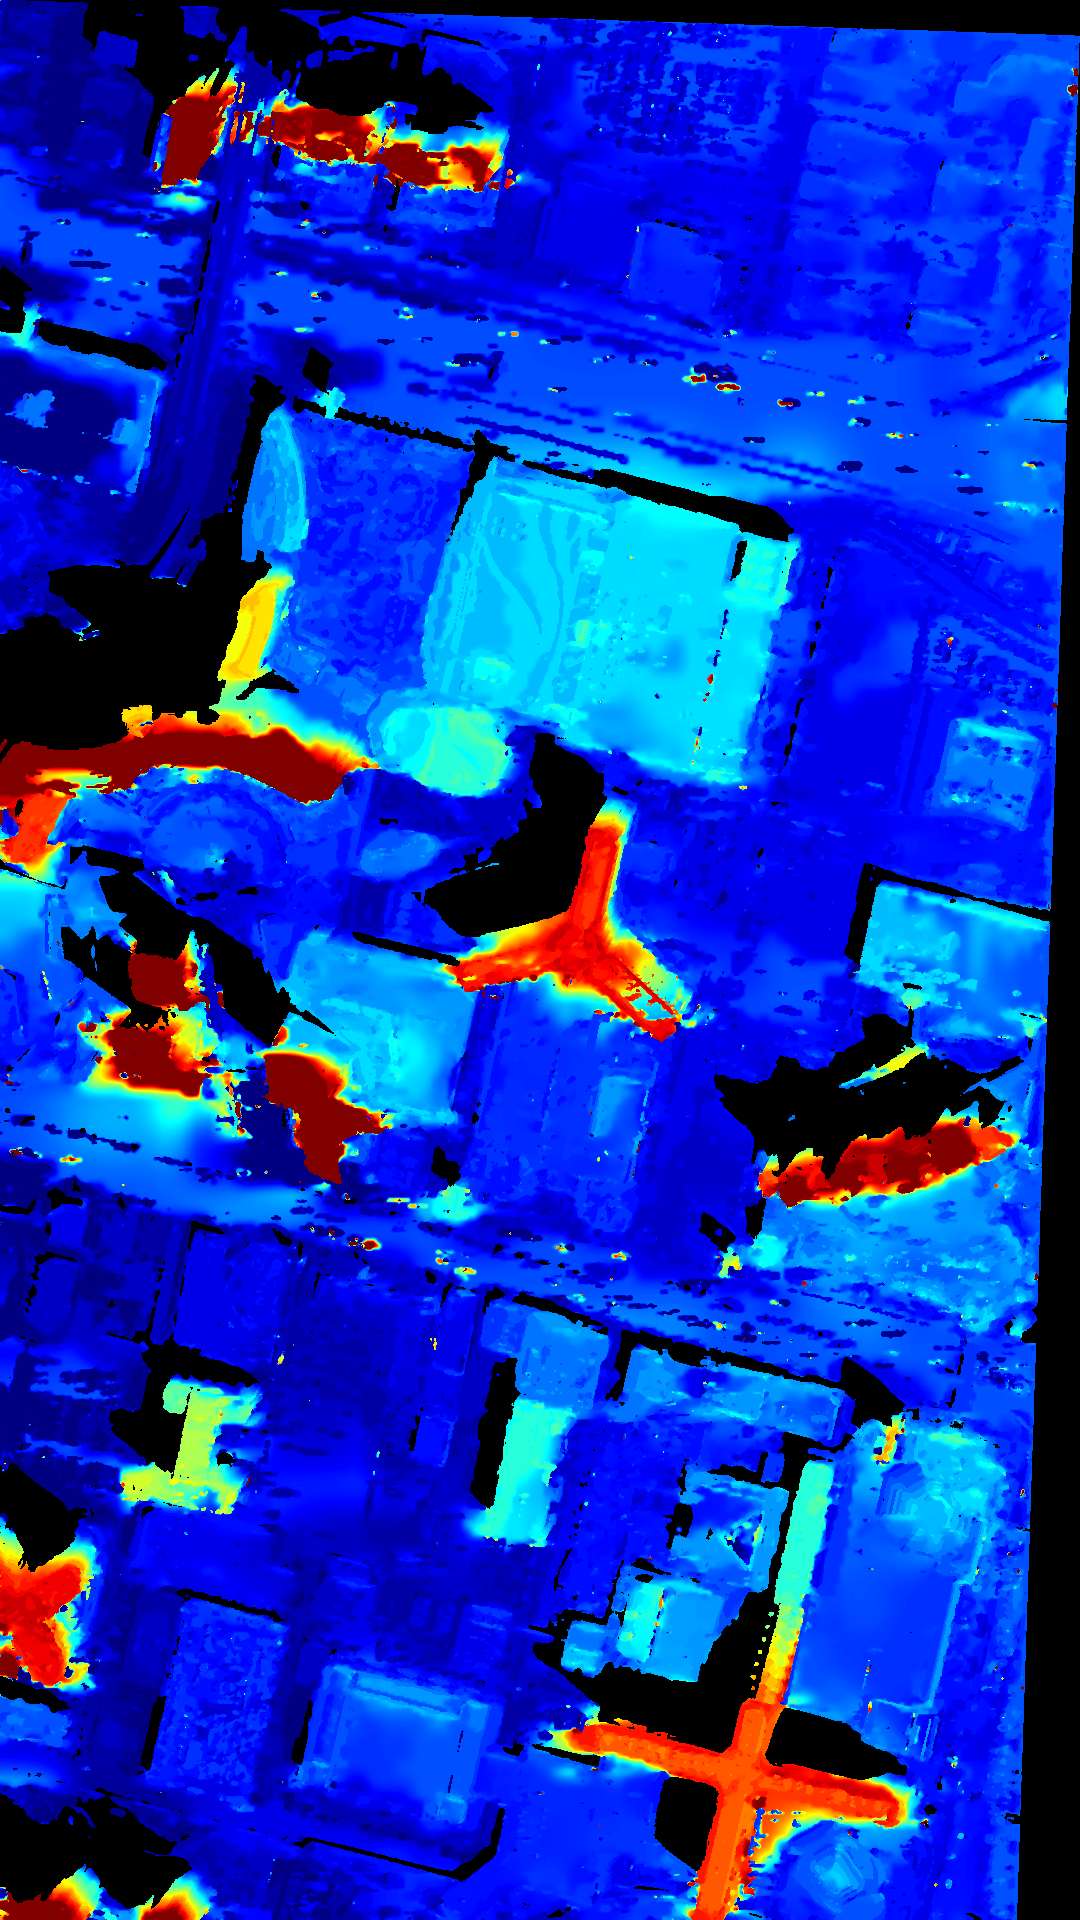
\includegraphics[height=8cm]{images/SkysatHR18_240/1521744514157_dmap_050.png}\\
 \vspace{-0.11em}
 %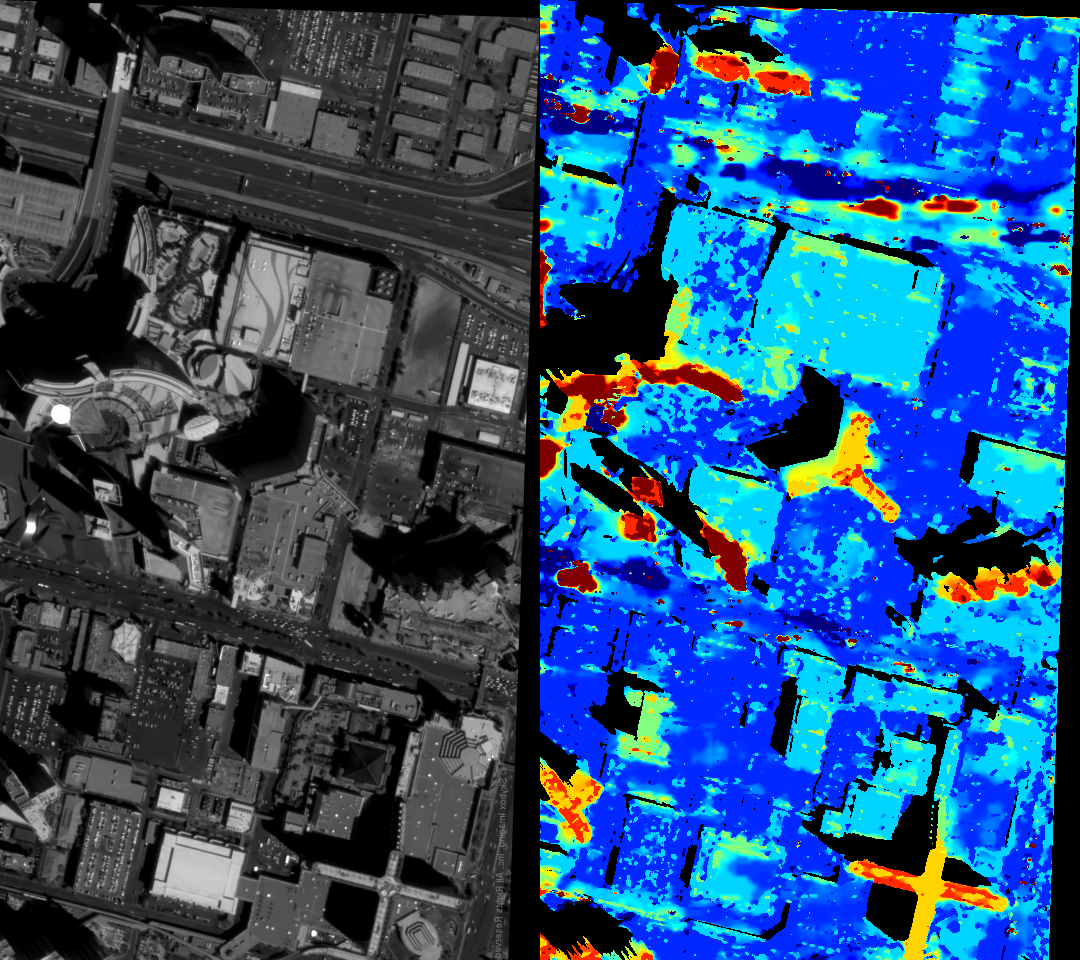
\includegraphics[height=8cm]{images/SkysatLR01_120/1521737975374_dmap_025.png}\hspace{-0.28em}
 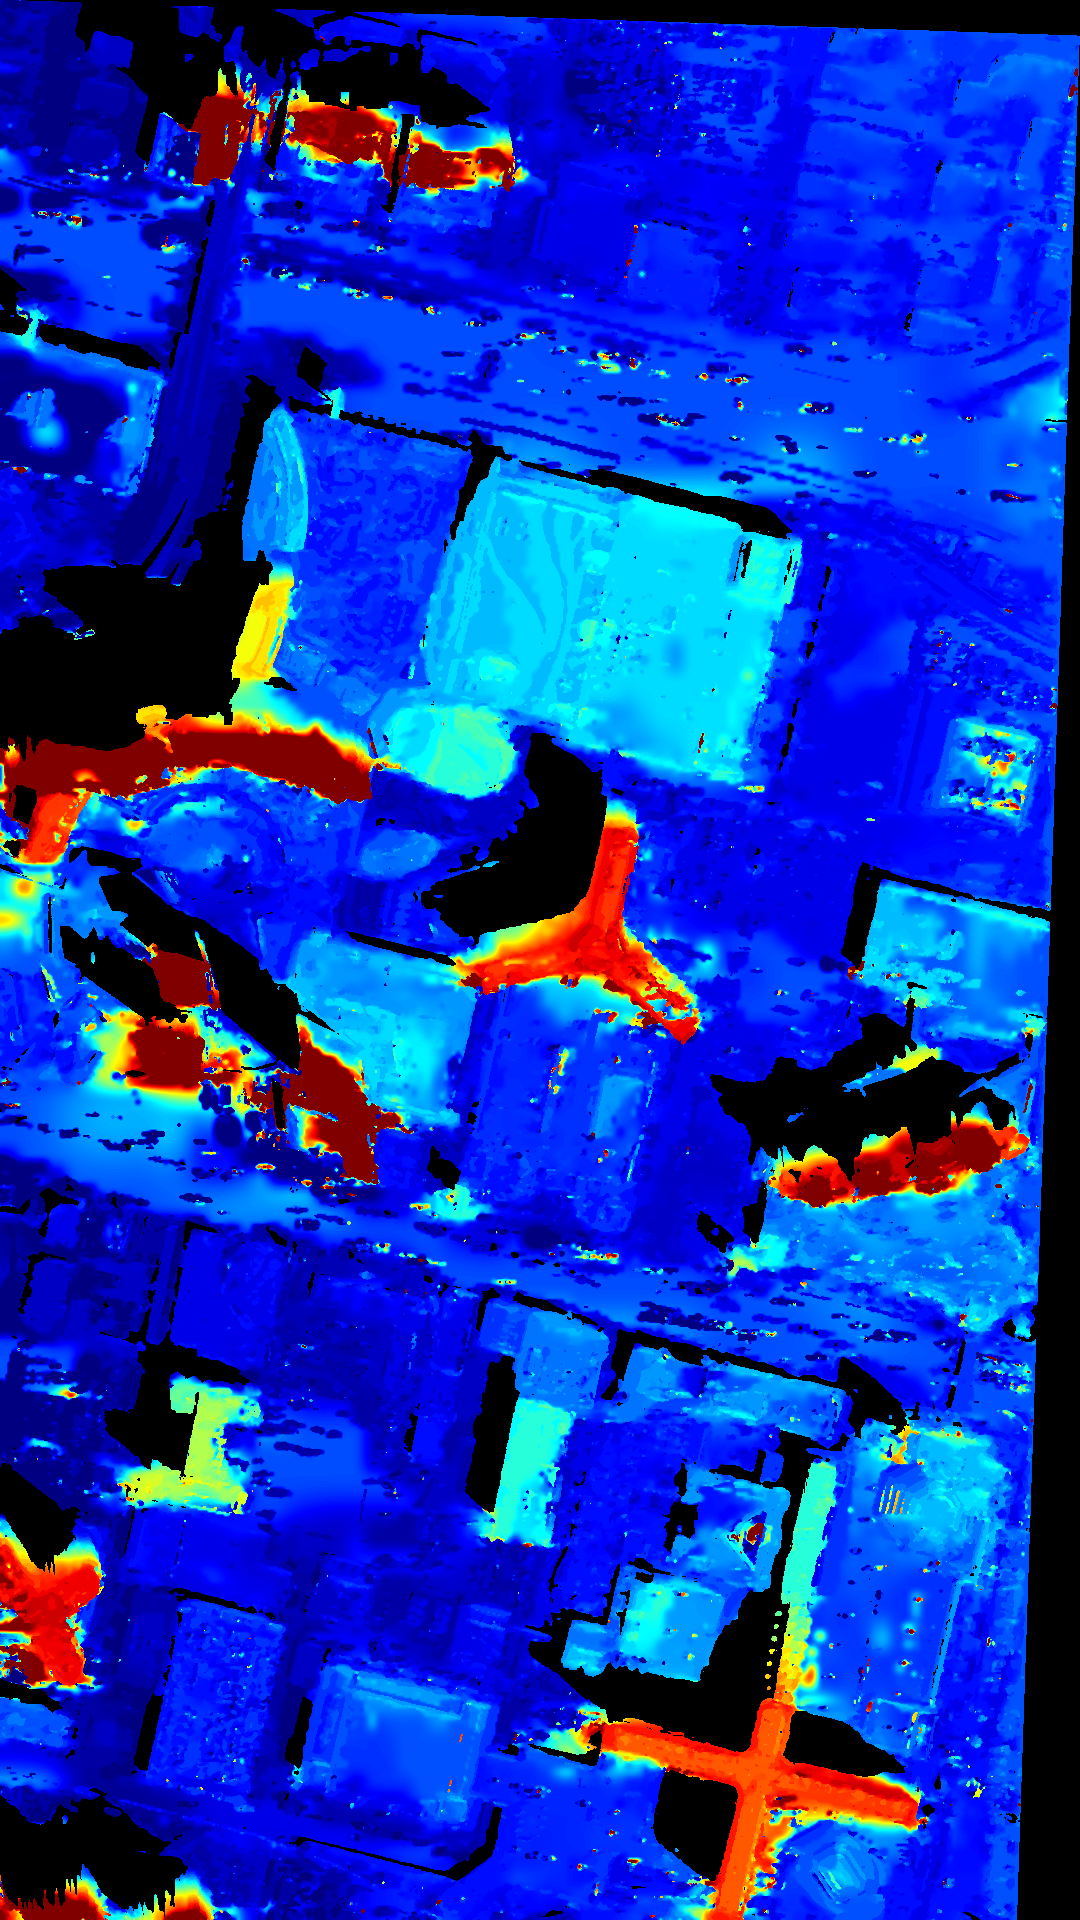
\includegraphics[height=8cm]{images/SkysatHR18_240/1521744514157_dmap_025.png}
 \caption{Influence of the resolution of the images. Original frame (left) SkysatLR18 $-1:4$ $[120]$ (middle) and SkysatHR18 $-1:4$ $[240]$ (right). Frame $50$ (top) and $25$ (bottom).}
 \label{fig:influenceres}
\end{figure}



% \section{Choice of the article and objective}
% 
% 
% We first investigated two different articles that describe two different methods for estimating depths maps from videos.
% \begin{itemize}
%  \item \cite{art:perez13:tvl1} describes an algorithm that estimates the optical flow given two images using a global optimization scheme minimizing a data attachment term and a regularization using the total variation of the flow. The idea is that the brightness $I$ of single points along their trajectories should be constant in time, leading to the optical flow constraint equation
%  \[ \nabla I \cdot \vect{u} + \Dpar{I}{t} = 0 \]
%  where $\vect{u}$ is the optical flow (the velocity vector field). The article then introduces a regularization on $\vect{u}$ (its total variation) and reformulates the problem in order to adapt to discrete sequences of images so that the attachent term consists in minimizing some $L^1$ term. In order to solve the subsequent global optimization problem, the authors propose a numerical scheme based on alternate optimization scheme. Finally, the authors investigate the influence of the several parameters of the algorithm -- noticeably the weight $\lambda$ of the data attachment term -- on the precision of the estimation of the optical flow and the sensitivity to noise.
%  
%  In our case, the optical flow computed with this algorithm could be interpreted as some disparity measurement. An interesting point is that the computation of the optical flow can be done on any pair of images, even if not rectified.
%  
%  \item \cite{art:kim13:lfields} describes a method for computing precise and exhaustive depth maps using ``light fields'', that is a dense set of images captures along a linear path. By concatenating one line of the rectified images together, one obtains an ``epipolar-plane image'' (EPI), in which a single scene point appears as a linear trace which slope is related to its distance to the camera. Thus, by estimating these slopes, one can reconstruct the depth of each point of the scene.
%  
%  The authors use very high definition images, so that the article includes several implementation details in order to ensure computational feasibility, both in terms of space (sparse representation of light fields) and computational power. For instance, they prefer local optimization near object boundaries and propagation to nearby areas in a fine-to-coarse approach to global optimization on the whole image. In the end, the method seems relatively fast, precise and robust to inconsistencies and outliers like noise or temporary occlusions.
% \end{itemize}


% We chose to work on the latter article. The objective of the project is then to implement the method presented by Kim et al. in \cite{art:kim13:lfields} and investigate how it performs with videos taken from SkySat. We will first investigate the case in which the images from the video are pre-rectified. Then we will investigate more complicated situations, for instance increasing the density of the images and considering non-pre-rectified sequences.

\clearpage
\bibliographystyle{plain}
\bibliography{bibliography}


\appendix
\section{Implementation details}


TODO (still need to clean code)


% C++


% Diagramme de classes


% Fonctions et minimal working example


\end{document}